% TODO: chỉnh lại hình ảnh cho đúng kiến trúc
% TODO: payload tiếng Việt là gì
\chapter{Yêu cầu và thiết kế hệ thống ứng dụng webfuzzer}
Chương này trình bày các yêu cầu cần đạt trong quá trình thiết kế - hiện thực và chi tiết kiến trúc của ứng dụng webfuzzer.
\section{Yêu cầu hiện thực}
Trong đề mục này, những yêu cầu tổng quan và chức năng của ứng dụng và cơ sở dữ liệu của webfuzzer sẽ được làm rõ. Công dụng chính của webfuzzer là để lưu trữ những điểm cuối ứng dụng web khả nghi, kiểm thử theo thiết lập có sẵn và lưu lại lịch sử kiểm thử chi tiết. Trong phạm vi luận văn này, chúng tôi chỉ tập trung vào giao diện người dùng (\acrfull{ui} - \acrshort{ui}), backend và cơ sở dữ liệu của ứng dụng webfuzzer, phần mở rộng Burp Suite đã được cung cấp và có tài liệu sẵn.
\subsection{Ứng dụng web}
Dưới đây là những yêu cầu tổng quan và chức năng của ứng dụng webfuzzer trong quá trình thiết kế và hiện thực backend và UI.
\subsubsection{Về tổng quan}
\begin{enumerate}
    \item Khả năng tiếp cận\\
    Backend và UI phải dễ dàng được tiếp cận được từ phía phần mở rộng Burp Suite và người dùng. Người dùng có thể tiếp cận mọi chức năng, giao diện lập trình ứng dụng (\acrlong{api} - \acrshort{api}) của ứng dụng và trước mắt chưa cần thiết phải có hệ thống phân quyền hay hạn chế việc này.
    \item Khả năng mở rộng\\
    Cấu hình kiểm thử ở phía backend phải linh hoạt, có thể được chỉnh sửa và thêm loại lỗ hổng bảo mật mới có thể được phát hiện theo cách tương tự. UI của ứng dụng nên được viết theo kiểu hướng thành phần (component-based) để có thể dễ dàng mở rộng bằng việc tái sử dụng các thành phần tương tự đã được lập trình trước.
    \item Hiệu năng\\
    Thời gian thực hiện một yêu cầu kiểm thử càng xấp xỉ (hoặc nhanh hơn) kiểm thử trên Burp Suite càng tốt. UI phải uyển chuyển, cung cấp được đầy đủ thông tin cần thiết để người dùng tiến hành kiểm thử và kiểm tra kết quả. Thời gian trả về kết quả khi gọi API không quá 1 giây cho một request trong điều kiện bình thường.
\end{enumerate}
\subsubsection{Về chức năng}
\begin{enumerate}
    \item Nhận và hiển thị \acrshort{http} request mẫu nhận được từ phần mở rộng Burp Suite\\
    Backend phải nhận được \acrshort{http} request mẫu được gửi từ phần ứng dụng của Burp Suite và lưu vào cơ sở dữ liệu, đồng thời UI phải hiển thị được những request mẫu đó thông qua việc tương tác với API của webfuzzer.
    \item Tùy chỉnh được cấu hình kiểm thử ứng với mỗi loại lỗ hổng bảo mật\\
    Cấu hình kiếm thử đối với từng lọai lỗ hổng phải có thể chỉnh sửa được (ít nhất là từ phía backend), đồng thời phải cung cấp API trả về cấu hình kiểm thử để hiển thị trên UI.
    \item Tạo và thực thi yêu cầu kiểm thử\\
    Dựa vào request mẫu và cấu hình kiểm thử hiển thị trên UI, người dùng phải dễ dàng tạo được yêu cầu kiểm thử trên UI thông qua việc chọn request mẫu và những loại lỗ hổng bảo mật cần kiểm thử. Sau đó người dùng có thể xem lại các thông số đó và tiến hành thực thi yêu cầu tương ứng.
    \item Xem kết quả kiểm thử\\
    Người dùng có thể xem lại kết quả kiểm thử trên UI, bao gồm các thông số, trạng thái, kết quả của mỗi yêu cầu kiểm thử cụ thể, kèm theo danh sách các payload phát hiện được mỗi loại lỗ hổng (nếu có). Đồng thời người dùng có thể dễ dàng lọc riêng những yêu cầu kiểm thử dương tính để xem xét thay vì hiển thị cả những yêu cầu âm tính.
\end{enumerate}
\subsection{Cơ sở dữ liệu}
Dưới đây là những yêu cầu tổng quan và chức năng của ứng dụng webfuzzer trong quá trình thiết kế và hiện thực một cơ sở dữ liệu nhanh và bền vững, đáp ứng được lưu cầu lưu trữ và truy xuất dữ liệu từ phía backend.
\subsubsection{Về tổng quan}
\begin{enumerate}
    \item Hạn chế trùng lặp dữ liệu\\
    Cơ sở dữ liệu phải tránh được tối đa việc lưu trữ các bản ghi hoặc thông tin trùng lặp, giữ cho kích thước của cơ sở dữ liệu càng nhỏ càng tốt.
    \item Khả năng mở rộng\\
    Lược đồ quan hệ và dữ liệu lưu trữ trong cơ sở dữ liệu cần có khả năng mở rộng cao, đặc biêt là những thông tin có độ dài không xác định trước được như kết quả kiểm thử, độ dài của request mẫu,...
    \item Hiệu năng\\
    Các câu truy vấn tới cơ sở dữ liệu phải có thời gian phản hồi trong khoảng chấp nhận được trong điều kiện bình thường, sao cho thỏa điều kiện thời gian phải hồi khi gọi API không quá 1 giây cho mỗi lời gọi API ở phía backend.
    \item Khả năng tương thích\\
    Việc cấu hình cơ sở dữ liệu, thiết lập các kết nối (connections) và truy vấn (queries) nên được hiện thực dễ dàng và hiệu quả trên ngôn ngữ lập trình phần backend của webfuzzer.
\end{enumerate}
\subsubsection{Về chức năng}
Cơ sở dữ liệu phải lưu trữ được đầy đủ và chính xác các thông tin của request mẫu bao gồm điểm cuối ứng dụng web mục tiêu, phương thức \acrshort{http}, cookies (nếu có) và các headers được gửi đến từ phần mở rộng Burp Suite; tương tự đối với các yêu cầu kiểm thử và kết quả kiểm thử tương ứng (nếu có).
\section{Trường hợp sử dụng}
Webfuzzer tập trung chủ yếu vào ba trường hợp sử dụng (use case) chính sau:
\begin{itemize}
    \item Trường hợp sử dụng 1: Gửi request mẫu từ phần mở rộng Burp Suite
    \begin{table}[ht]
        \centering
        \caption{Trường hợp sử dụng 1}
        \label{tab:use-case-1}
        \begin{tabular}[ht]{lll}
            \toprule[1pt]\midrule[0.3pt]
                \textbf{Đối tượng tương tác}& &Người dùng, phần mở rộng Burp Suite, \acrshort{ui} webfuzzer\\
            \midrule
                \textbf{Ranh giới hệ thống}& &Máy tính cá nhân của người dùng\\
            \midrule
                {}& &Backend và \acrshort{ui} của ứng dụng webfuzzer đang họat động,\\
                \textbf{Điều kiện trước}{}& &phần mềm Burp Suite có cài đặt sẵn phần mở rộng\\
                {}& &và trình duyệt web có thiết lập proxy sẵn\\
            \midrule
                {}& &Người dùng chọn và gửi request mẫu cần kiểm thử đến\\
                \textbf{Luồng thực thi}& &địa chỉ IP:port của ứng dụng. Webfuzzer sẽ phân giải request đó,\\
                {}& &lưu vào cơ sở dữ liệu và hiển thị lên giao diện người dùng\\
            \midrule
                {}& &Request mẫu được hiển thị trong danh sách \\
                \textbf{Điều kiện sau}& &trên giao diện webfuzzer sau thao tác gửi request\\
                {}& &và làm mới từ người dùng\\
            \midrule[0.3pt]\bottomrule[1pt]
        \end{tabular}
    \end{table}
    \FloatBarrier
    \item Trường hợp sử dụng 2: Tạo yêu cầu kiểm thử một điểm cuối ứng dụng web
    \begin{table}[ht]
        \centering
        \caption{Trường hợp sử dụng 2}
        \label{tab:use-case-2}
        \begin{tabular}[ht]{lll}
            \toprule[1pt]\midrule[0.3pt]
                \textbf{Đối tượng tương tác}& &Người dùng, giao diện người dùng webfuzzer\\ 
            \midrule
                \textbf{Ranh giới hệ thống}& &Máy tính cá nhân của người dùng\\
            \midrule
                \textbf{Điều kiện trước}& &Backend và \acrshort{ui} của ứng dụng webfuzzer đang họat động\\
            \midrule
                {}& &Người dùng chọn request mẫu từ danh sách đang hiển thị,\\
                \textbf{Luồng thực thi}& &sau đó chọn loại lỗ hổng cần kiểm thử\\
                {}& &và nhấn nút ``\textbf{Create fuzz request}''\\
            \midrule
                \textbf{Điều kiện sau}& &Yêu cầu kiểm thử tương ứng xuất hiện\\
                {}& &trong trang \textbf{Result} trên giao diện webfuzzer\\
            \midrule[0.3pt]\bottomrule[1pt]
        \end{tabular}
    \end{table}
    \FloatBarrier
    \item Trường hợp sử dụng 3: Xem kết quả kiểm thử theo thời gian
    \begin{table}[ht]
        \centering
        \caption{Trường hợp sử dụng 3}
        \label{tab:use-case-3}
        \begin{tabular}[ht]{lll}
            \toprule[1pt]\midrule[0.3pt]
                \textbf{Đối tượng tương tác}& &Người dùng, giao diện người dùng webfuzzer\\ 
            \midrule
                \textbf{Ranh giới hệ thống}& &Máy tính cá nhân của người dùng\\
            \midrule
                \textbf{Điều kiện trước}& &Backend và \acrshort{ui} của ứng dụng webfuzzer đang họat động\\
            \midrule
                \textbf{Luồng thực thi}& &Người dùng chọn trang \textbf{Result} để xem kết quả kiểm thử\\
                {}& &hoặc chọn một yêu cầu cụ thể để xem chi tiết\\
            \midrule
                \textbf{Điều kiện sau}& &Người dùng xem được tổng quan và chi tiết kết quả của mỗi\\
                {}& &yêu cầu kiểm thử. Đồng thời cho phép người dùng tái hiện lại\\
                {}& &request gây lỗi trên điểm cuối ứng dụng web mục tiêu\\
            \midrule[0.3pt]\bottomrule[1pt]
        \end{tabular}
    \end{table}
\end{itemize}
Bảng \ref{tab:use-case-1} thể hiện trường hợp sử dụng đầu tiên, cụ thể là khi người dùng muốn gửi request mẫu cần kiểm thử đến ứng dụng để hiển thị trên giao diện người dùng webfuzzer. Người dùng chọn request mẫu và vị trí tham số theo nhu cầu kiểm thử trên phần mở rộng Burp Suite, sau đó gửi đến địa chỉ IP:port đang triển khai ứng dụng webfuzzer (sẽ được trình bày chi tiết ở \textbf{Phụ lục A}). Sau đó nội dung của request mẫu này sẽ được hiển thị trên giao diện để người dùng kiểm tra và tạo yêu cầu kiểm thử theo một số lỗ hổng bảo mật.\par
Bảng \ref{tab:use-case-2} thể hiện trường hợp người dùng muốn tạo yêu cầu kiểm thử một request mẫu cụ thể với một số loại lỗ hổng. Người dùng chỉ việc chọn request mẫu trong danh sách và đánh dấu loại lỗ hổng cần kiểm thử và nhấn nút ``\textbf{Create fuzz request}''. Yêu cầu kiểm thử sẽ được đưa vào hàng đợi thực thi, đồng thời trạng thái và kết quả kiểm thử theo thời gian của yêu cầu này sẽ được hiển thị trong trang \textbf{Result} trên giao diện ứng dụng.\par
Trường hợp sử dụng 3 được thể hiện trong Bảng \ref{tab:use-case-3}. Trong trường hợp này, người dùng có thể xem chung kết quả của một số yêu cầu kiểm thử gần đây nhất hoặc xem chi tiết kết quả của một yêu cầu bất kì theo thời gian thực bao gồm kết quả tổng quát, những payload/biểu thức chính quy phát hiện ra lỗi, đồng thời cho phép người dùng gửi lại request mẫu kèm theo những payload đó để tái hiện lại bằng chứng (\acrshort{poc}) mắc lỗi của ứng dụng web mục tiêu.
\section{Công nghệ sử dụng}
Đề mục này trình bày tóm tắt những ngôn ngữ lập trình, công nghệ, công cụ được chọn để hiện thực ứng dụng webfuzzer. Những công nghệ này được lựa chọn dựa trên những nghiên cứu nền trong quá trình thực hiện luận văn. Chúng tương thích, hỗ trợ lẫn nhau và thích hợp trong việc thỏa mãn những yêu cầu hiện thực đã đề ra.\par
\textbf{Node.js} là một nền tảng phát triển ứng dụng độc lập được xây dựng trên Javascript Runtime của trình duyệt Chrome, thường được sử dụng để xây dựng các ứng dụng web một cách nhanh chóng và dễ dàng mở rộng. Phần lõi bên dưới của Node.js được viết hầu hết bằng C++ nên tốc độ xử lý và hiệu năng khá cao. Nhìn chung Node.js là một nền tảng rất thích hợp trong việc nhanh chóng xây dựng những ứng dụng web đa chức năng với hiệu năng cao, thích hợp với các startup hay luận văn tốt nghiệp này vì những lý do sau.
\begin{itemize}
    \item Node.js chạy đa nền tảng phía Server, sử dụng kiến trúc hướng sự kiện (event-driven), cơ chế non-blocking I/O làm cho nó nhẹ và hiệu quả.
    \item Ứng dụng viết bằng Node.js có thể chạy được ở bất kỳ hệ điều hành Mac – Windows – Linux.
    \item Cộng đồng Node.js rất lớn, hơn một triệu ba trăm nghìn gói thư viện (package) được cung cấp hoàn toàn miễn phí trên trang \href{https://www.npmjs.com/}{\textit{https://www.npmjs.com/}}, hỗ trợ trải dài trên nhiều lĩnh vực lập trình từ đại trà đến đặc thù.
    \item Các ứng dụng Node.js đáp ứng tốt thời gian thực và chạy đa nền tảng, đa thiết bị.
\end{itemize}
\textbf{Express.js} là một khung thức nhỏ, linh hoạt được xây dựng trên nền tảng Node.js. Nhiều khung thức nổi tiếng trên nền Node.js hiện đang sử dụng Express.js như \textbf{Sails}, \textbf{Feathers},... Express.js được xây dựng dựa trên rất nhiều gói thư viện bổ trợ và cung cấp thêm nhiều tính năng để lập trình viên tốt hơn, không làm giảm tốc độ vốn có của Node.js. Trong phạm vi luận văn này, Express.js được sử dụng như một bộ định tuyến (routing), đảm nhiệm việc phản hồi thông tin lại cho người dùng khi họ yêu cầu đến những điểm cuối của ứng dụng webfuzzer. Những yêu cầu này thuộc dạng HTTP request bao gồm đường dẫn đến điểm cuối, phương thức request (GET, POST, DELETE, PUT,...) và các tham số cần thiết. \par
\textbf{React.js} là một thư viện hỗ trợ lập trình giao diện người dùng phổ biến trên ngôn ngữ Javascript. Một ứng dụng React.js được xây dưng xung quanh các thành phần (component) với khả năng tái sử dụng cao, thay vì dựa vào bản mẫu (template) như các thư viện lập trình \acrshort{ui} khác, cho phép nhúng mã \acrshort{html} trong mã Javascript nhờ vào JSX. JSX có ba điểm nổi bật chính.
\begin{itemize}
    \item Nhanh hơn. JSX thực hiện nhiều biện pháp tối ưu hóa trong khi biên dịch sang mã Javacsript. Việc thực thi các mã JSX này tốn ít thời gian hơn so với một mã tương đương viết trực tiếp bằng Javascript.
    \item An toàn hơn. JSX được biên dịch trước khi chạy, giống như các ngôn ngữ tĩnh khác như Java, C++,... Vì thế các lỗi nếu có sẽ được phát hiện ngay trong quá trình biên dịch.
    \item Dễ sử dụng hơn. JSX được viết dựa trên Javascript, vì vậy rất dễ dàng để các lập trình viên Javascript như chúng tôi có thể hiểu và sử dụng.
\end{itemize}
\textbf{Burp Suite} \parencite{burpsuite} là một khung thức kiểm thử thâm nhập (penetration testing framework) ứng dụng web trên nền Java, được cung cấp và phát triển bởi PortSwigger và đã trở thành bộ công cụ tiêu chuẩn được dùng trong công nghiệp bởi những kĩ sư an toàn thông tin. Công cụ này hỗ trợ nhận diện lỗ hổng bảo mật và xác thực các véc tơ tấn công vào ứng dụng web.
\begin{figure}[H]
  \centering
    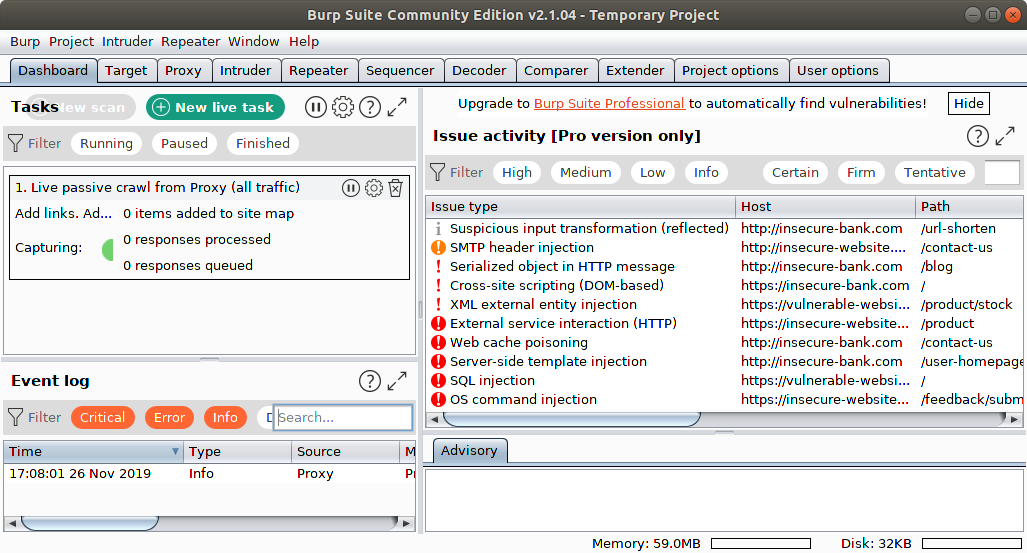
\includegraphics[width=\textwidth,keepaspectratio=true]{images/burp-suite-usage.png}
  \caption{Giao diện chính của công cụ Burp Suite}
  \label{fig:burp-suite-usage}
\end{figure}
Trong phạm vi luận văn này, Burp Suite vừa đóng vai trò như một proxy trung gian (interception proxy) can thiệp vào quá trình gửi \acrshort{http} request đến ứng dụng web mục tiêu, vừa đóng vai trò của một người trung gian (man in the middle - MITM) hỗ trợ chúng tôi phân tích, chỉnh sửa và chuyển tiếp request mẫu đó tới ứng dụng webfuzzer đồng thời cung cấp dữ liệu đối chứng trong quá trình kiểm thử tính đúng đắn và hiệu quả của ứng dụng.\par
\textbf{MySQL} là một hệ quản trị cơ sở dữ liệu mã nguồn mở, được sử dụng phổ biến trên thế giới vì tốc độ cao, sự ổn định, dễ sử dụng và khả năng hoạt động được trên nhiều hệ điều hành của nó. MySQL là một hệ quản trị cơ sở dữ liệu quan hệ, sử dụng ngôn ngữ truy vấn có cấu trúc (\acrlong{sql} - \acrshort{sql}). Đặc biệt MySQL có tính sẵn sàng và nhất quán cao theo mô hình CAP (Consistency - Availability - Partition tolerance), có sẵn thư viện tương tác được viết bằng Node.js và tương thích tốt với các hệ điều hành Windows, Linux, Mac OS X. Dựa vào những yếu tố trên, MySQL rất phù hợp trong việc hiện thực một cơ sở dữ liệu dựa trên những công nghệ và yêu cầu đã đề ra.
\section{Thiết kế kiến trúc hệ thống}
Đề mục này mô tả thiết kế chi tiết của kiến trúc hệ thống ứng dụng webfuzzer, bao gồm ba thành phần backend, \acrshort{ui} và cơ sở dữ liệu của ứng dụng.
\subsection{Backend}
Hai thành phần quan trọng nhất của backend 
\subsubsection{Cấu hình và mô-đun kiểm thử}
Dựa vào cách thức phát hiện lỗ hổng bằng thời gian phản hồi \acrshort{http} request và sự trùng khớp nội dung của response trả về, đối với mỗi loại lỗ hổng, chúng tôi xây dựng cấu hình kiểm thử bao gồm các thuộc tính sau. 
\begin{itemize}
    \item \textbf{label} là tên của lỗ hổng đang kiểm thử, dùng trong việc hiển thị trên giao diện và ghi nhật kí hoạt động.
    \item \textbf{time} là thời gian tối thiểu để một request kiểm thử trả về response, nếu thời gian phản hồi này lớn hơn giá trị của thuộc tính \textbf{time} thì được coi là phát hiện thành công lỗ hổng time-based \acrshort{sqli}. Thuộc tính này có thể là số giây cụ thể hoặc một chuỗi rỗng trong trường hợp người dùng không muốn giới hạn thời gian.
    \item \textbf{match} là một mảng các chuỗi để so trùng trên \acrshort{http} response, điểm cuối của ứng dụng web mục tiêu sẽ bị coi là có lỗ hổng nếu response trả về có chứa một trong những chuỗi này. 
    \item \textbf{payloadFile} là đường dẫn tập tin chứa các payload kiểm thử. Mặc định các payload này được chứa trong thư mục \texttt{payloads} trong thư mục gốc của mã nguồn backend và phân loại theo lỗ hổng bảo mật.
    \item \textbf{matchFile} là tập tin chứa các chuỗi để so trùng tương tự như thuộc tính \textbf{match} của cấu hình.
    \item \textbf{regex} là biểu thức chính quy dùng để phát hiện các chuỗi đáng ngờ trong \acrshort{http} response trả về, tương tự như thuộc tính \textbf{match}, điểm cuối của ứng dụng web mục tiêu sẽ bị coi là có lỗ hổng nếu response trả về khớp với các biểu thức chính quy này. Các biểu thức chính quy không chỉ bao gồm được các chuỗi để so trùng mà còn gồm cả các thông báo lỗi từ hệ điều hành, hệ quản trị cơ sở dữ liệu hay của chính ứng dụng web mục tiêu. Điều này gợi ý cho chúng tôi về những tiềm năng khai thác xa hơn, ngoài những lỗ hổng bảo mật ở tầng ứng dụng.
\end{itemize}
Việc thiết kế mô-đun kiểm thử sẽ được hiện thực dựa trên nguyên tắc hoạt động của chức năng \textbf{Intruder} trên Burp Suite, sử dụng loại tấn công \textbf{Sniper} như đã đề cập ở \textbf{Chương 4}, gồm các mô-đun nhỏ và các bước tuần tự như sau.
\begin{enumerate}
    \item Mô-đun phân tích request (\texttt{requestParser}) nhận vào \acrshort{http} request mẫu và cấu hình kiểm thử. Mô-đun này tiến hành đọc danh sách các payload từ thuộc tính \texttt{payloadFile} của cấu hình kiểm thử. Sau đó xác định từng vị trí thay thế payload riêng lẻ trong request mẫu (ở dạng chuỗi), được đánh dấu bằng cặp kí tự ``\$'' để thay thế lần lượt từng payload vào từng vị trí. Kết quả trả về một danh sách các \acrshort{http} request mẫu có chứa payload.
    \item Mô-đun xây dựng request kiểm thử (\texttt{requestBuilder}) nhận vào danh sách request chứa payload ở trên. Mô-đun này lần lượt xây dựng \acrshort{http} request kiểm thử đầy đủ dựa trên các thành phần \texttt{url, headers, cookies, data, method} của từng chuỗi request mẫu trong danh sách. Sau đó các request kiểm thử này lần lượt được gửi đến ứng dụng web mục tiêu.
    \item Các mô-đun kiểm thử (\texttt{fuzzer}) sẽ kiểm tra thời gian phản hồi và so trùng nội dung \acrshort{http} response trả về dựa trên cấu hình kiểm thử để xác định khả năng có lỗ hổng của điểm cuối ứng dụng web mục tiêu. 
    \item Trong trường hợp mô-đun lưu trữ kết quả kiểm thử (\texttt{updateFuzzingLog}) lưu lại (hoặc cập nhật) loại lỗ hổng mà điểm cuối của ứng dụng web mục tiêu mắc phải kèm theo những payload phát hiện được lỗ hổng tương ứng vào cơ sở dữ liệu.
\end{enumerate}
\subsubsection{Giao diện lập trình ứng dụng - \acrshort{api}}
Giao diện lập trình ứng dụng của webfuzzer sẽ được điều hướng thông qua chức năng định tuyến (routing) được hỗ trợ bởi khung thức Express.js và hiện thực bằng các lớp trình điều khiển (controller). Các lớp này cung cấp các phương thức để tương tác với cơ sở dữ liệu, trả về thông tin và tiến hành kiểm thử ở phía backend. \acrshort{ui} của webfuzzer sẽ tạo \acrshort{http} request gọi đến đường dẫn \acrshort{api} kèm theo những tham số cần thiết, các phương thức này sẽ xử lý những request đó và trả về response dưới dạng đối tượng JSON. Các lớp trình điều khiển và các phương thức trong đó hoạt động độc lập với nhau, được phân loại theo chức năng như sau.
\begin{itemize}
    \item Lớp \textbf{BurpController} xử lý các yêu cầu liên quan đến \acrshort{http} request mẫu, bao gồm nhận request từ phía phần mở rộng Burp Suite và trả về danh sách các request mẫu đã lưu.
    \item Lớp \textbf{TargetController} đảm nhiệm việc tạo yêu cầu kiểm thử, truy vấn cấu hình kiểm thử và thông tin của các yêu cầu kiểm thử. Các phương thức trong lớp này không chỉ trả về một danh sách các yêu cầu kiểm thử được lọc ra theo nội dung tìm kiếm hoặc phân loại theo kết quả kiểm thử có lỗ hổng hay không mà còn có thể trả về thông tin chi tiết của một yêu cầu kiểm thử đơn lẻ.
    \item Lớp \textbf{FuzzController} cung cấp các phương thức thực thi yêu cầu kiểm thử theo ID hoặc một yêu cầu ngẫu nhiên đã được tạo.
\end{itemize}
Mỗi phương thức trong các lớp trình điều khiển này thực hiện những công việc tương ứng với chức năng của một \acrshort{api}. Cụ thể, Bảng \ref{tab:api-design} dưới đây mô tả kiến trúc giao diện lập trình ứng dụng ở phía backend của webfuzzer.
\FloatBarrier
\begin{table}[ht]
    \centering
    \caption{Kiến trúc giao diện lập trình ứng dụng của webfuzzer backend}
    \label{tab:api-design}
    \begin{tabular}[ht]{cccl}
        \toprule[1pt]\midrule[0.3pt]
            \textbf{Lớp điều khiển}&\textbf{Tên phương thức}&\textbf{Đường dẫn API}&\textbf{Mô tả}\\ 
        \midrule
            {}&receiveTargetFromBurp&\colorbox{gray!30}{\texttt{POST /}}&Nhận request mẫu từ\\
            BurpController&{}&{}& phần mở rộng Burp Suite\\
            \addlinespace
            {}&getAllEndpoint&\colorbox{gray!30}{\texttt{GET /}}&Truy vấn danh sách các \\
            {}&{}&{}&request mẫu đã nhận\\
            \midrule[0.3pt]
            {}&createFuzzRequest&\colorbox{gray!30}{\texttt{POST /target}}&Tạo yêu cầu kiểm thử\\
            \addlinespace
            {}&retrieveRequestInfo&\colorbox{gray!30}{\texttt{GET /target}}&Truy vấn một yêu cầu\\
            {}&{}&{}& kiểm thử theo ID\\
            \addlinespace
            {}&getRequestList&\colorbox{gray!30}{\texttt{GET /target/list}}&Truy vấn danh sách các\\
            TargetController&{}&{}&yêu cầu kiểm thử\\
            \addlinespace
            {}&getVulnTypes&\colorbox{gray!30}{\texttt{GET /target/configs}}&Truy vấn danh sách\\
            {}&{}&{}&cấu hình kiểm thử\\
            \addlinespace
            {}&searchUrl&\colorbox{gray!30}{\texttt{GET /target/search}}&Lọc yêu cầu kiểm thử\\
            {}&{}&{}&theo \acrshort{url}\\
            \midrule[0.3pt]
            {}&executeFuzzRequest&\colorbox{gray!30}{\texttt{GET /fuzz/}}&Thực thi một yêu cầu\\
            FuzzController&{}&{}&kiểm thử theo ID\\
            \addlinespace
            {}&executeSubmittedRequest&\colorbox{gray!30}{\texttt{GET}}&Thực thi một yêu cầu\\
            {}&{}&\colorbox{gray!30}{\texttt{/fuzz/free-request}}&kiểm thử đã tạo\\
        \midrule[0.3pt]\bottomrule[1pt]
    \end{tabular}
\end{table}
% TODO: Viết phần cấu trúc chương trình này nếu có thời gian
\subsubsection{Cấu trúc chương trình}
\begin{itemize}
    \item Quản lý việc tương tác với cơ sở dữ liệu
    \item 
\end{itemize}
\subsection{Giao diện người dùng}
% \begin{enumerate}[label*=\arabic*.]
%     \item 
% \end{enumerate}
Giao diện của ứng dụng webfuzzer sẽ có hai trang web chính, bao gồm các thành phần như mô tả sau.
\begin{enumerate}
    \item Bảng điều khiển (Dashboard) để người dùng tạo yêu cầu kiểm thử.
    \begin{itemize}
        \item 
    \end{itemize}
    \item Kết quả kiểm thử (Result) để người dùng thực thi và kiểm tra kết quả kiểm thử.
    \begin{itemize}
        \item 
    \end{itemize}
\end{enumerate}
\subsection{Cơ sở dữ liệu}
Nhằm đảm bảo mục đích lưu trữ các \acrshort{http} request mẫu, yêu cầu và kết quả kiểm thử, cơ sở dữ liệu của ứng dụng nên tách ra làm ba bảng chứa các đối tượng trên, tạm gọi lần lượt là các bảng \texttt{Endpoint, Request, Result}. Đối tượng chính là sẽ là bảng \texttt{Request}, chứa request mẫu, cấu hình (nếu có thể), các loại lỗ hổng cần kiểm thử, kết quả kiểm thử và một số thông tin khác. Một request mẫu có thể được kiểm thử nhiều lần tùy theo nhu cầu của người dùng nên ta tách \texttt{Endpoint} ra thành một bảng riêng, bảng \texttt{Request} lúc này sẽ có một trường tham khảo đến khóa chính của bảng \texttt{Endpoint} để tránh tình trạng dư thừa dữ liệu. Tương tự, bảng \texttt{Result} chứa kết quả kiểm thử cũng nên được tách riêng và thiết lập quan hệ khóa ngoài với bảng \texttt{Request} để dễ dàng thay đổi và mở rộng sau này.\par
Ngoài ra, có một phần dữ liệu cần lưu trữ thuộc kiểu đối tượng JSON (JavaScript Object Notation) ở phía backend, một kiểu dữ liệu mở trong Node.js và Javascript, được cấu thành từ nhiều cặp thuộc tính - giá trị. MySQL không hỗ trợ lưu trữ trực tiếp kiểu dữ liệu đối tượng JSON này nên các giá trị có kiểu này cần được chuỗi hóa ở phía backend trước khi gửi đến cơ sở dữ liệu. Vì lý do đó, một số trường tương ứng trong các bảng sẽ có kiểu chuỗi (string) để lưu trữ chúng.